% !TEX root =../thesis-letomes.tex

\chapter{Literature Overview}
\section{1988-2014: LETOs to the Moon and Speculations on an Interplanetary Network of LETOs}
In traditional Hohmann transfer orbits, the spacecraft is moved between two orbits around a central body along an elliptical as in \cref{fig:hohmann}. However when rendezvousing with another body at the arrival orbit, a breaking maneuver is required (as opposed to a speeding up maneuver as depicted in \cref{fig:hohmann}). It is this breaking maneuver that low energy transfer orbits attempt to avoid. This is done by travelling between bodies along regions\footnote{also called a ``weak stability boundary'', this is a region around any large body where objects will be ``weakly captured'' by the body orbited. Therefore LETOs are also known a ``weak stability boundary trajectories''} near their Lagrange points\footnote{Lagrange points are points of equilibrium in a two-body system in their rotating non-inertial frame of reference. For a great animation showing these, see the bottom of \url{https://leancrew.com/all-this/2016/08/lagrange-points-redux/}} of minimum energy, see \cref{fig:lagrange-points-energy-contour-lines}. LETOs allow us to trade a longer trip time with lower delta-v (and fuel) requirements by intentionally passing through these regions and by coming in at just at just the right angle and velocity vector.

\begin{figure}[ht]
    \centering
    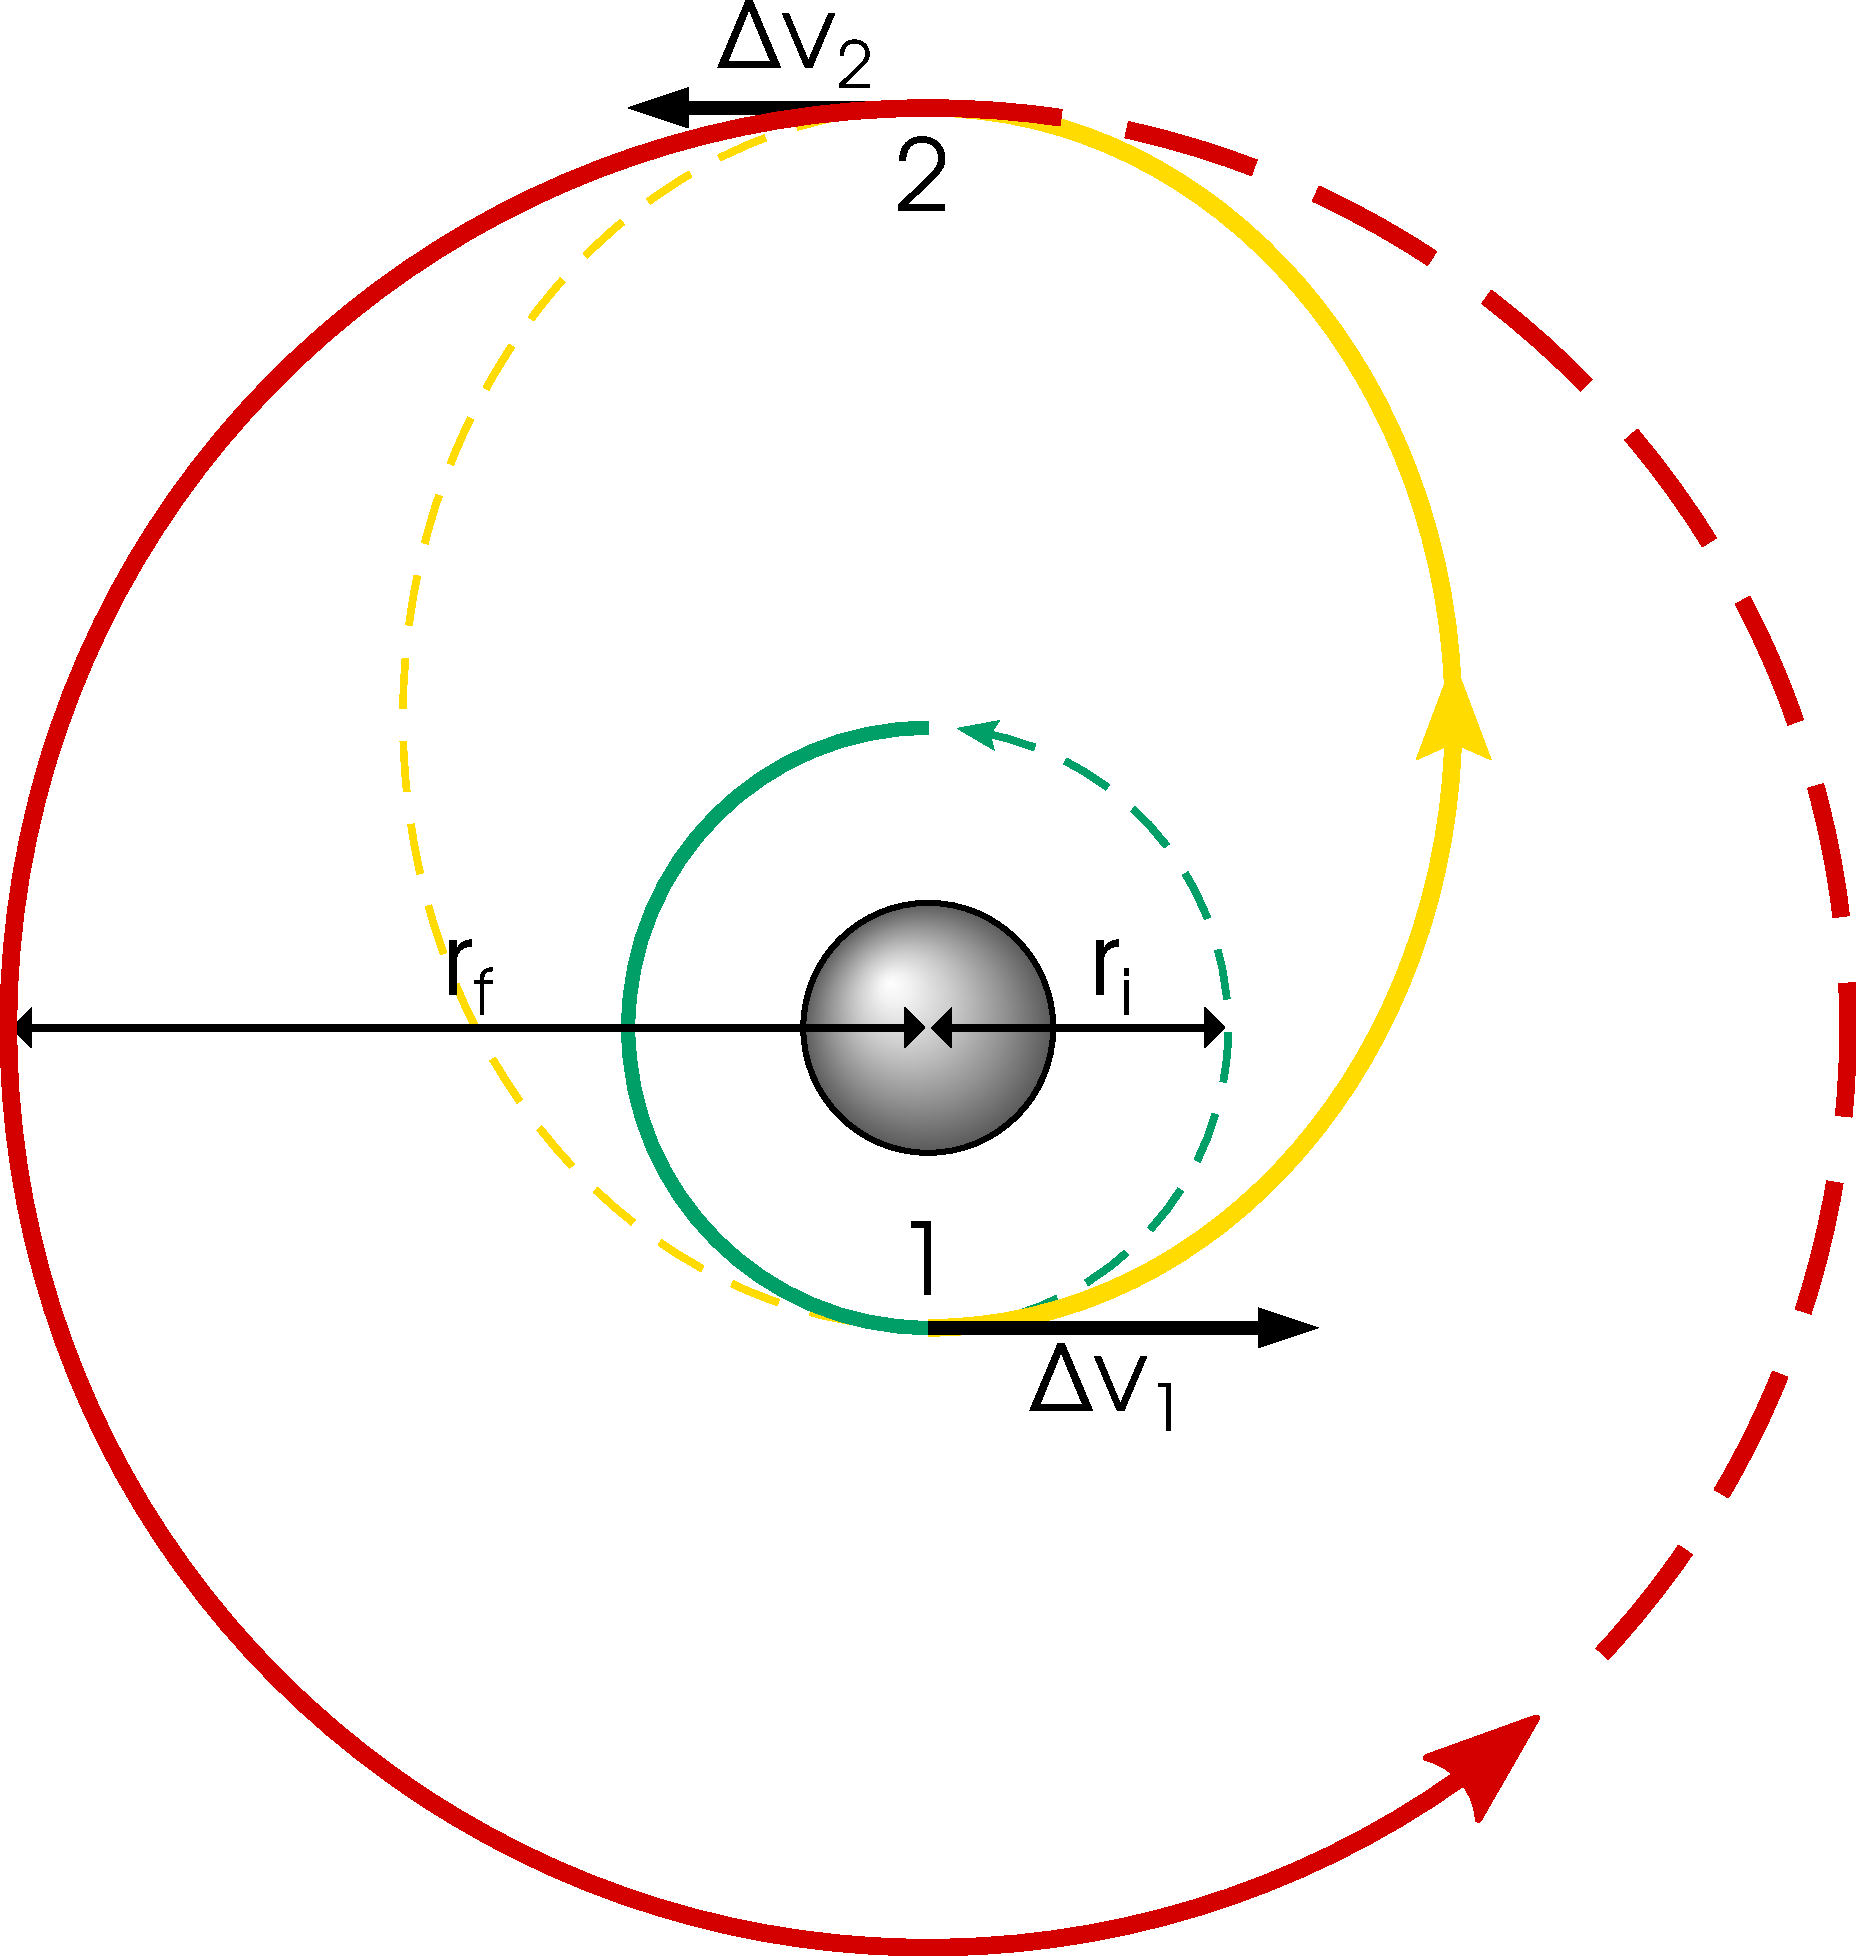
\includegraphics[width=0.4\linewidth]{fig/hohmann.pdf}
    \caption{Hohmann Transfer orbit that brings the satellite from one circular orbit around a central body to another circular orbit using two burns (Image: \cite{Leafnode} (modified)).}
    \label{fig:hohmann}
\end{figure}

\begin{figure}[ht]
    \centering
    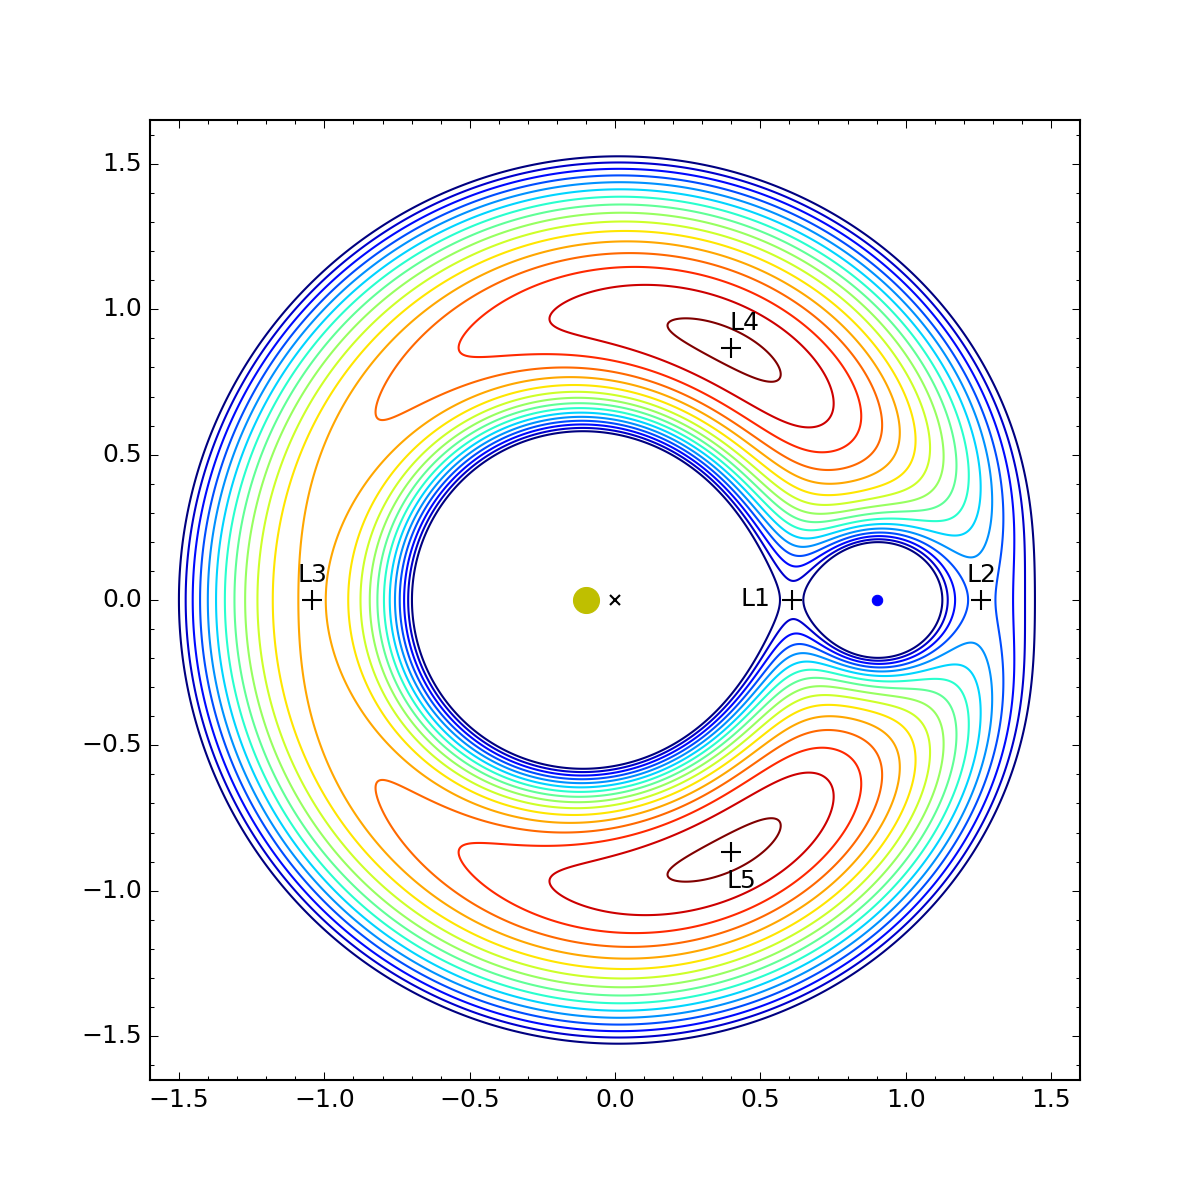
\includegraphics[width=0.65\linewidth]{fig/lagrange-points-energy-contour-lines.png}
    \caption{Contour lines of potential energy and Lagrange points of a two-body system. LETOs go through the region along L1 and L2 for capture at the smaller body or lowest energy travel to the solar system beyond (Image: \cite{Drang}).}
    \label{fig:lagrange-points-energy-contour-lines}
\end{figure}
Low energy transfer orbits (also known as ballistic capture) can be traced back to conference proceedings in in 1987, where Edward Belbruno first discovered it as a cheaper way to the Moon under the constraint of using just electric propulsion, a class of engines known for their high efficiency but low thrust. It turned out to be possible in theory, albeit the trip would take nearly 2 years \cite{Belbruno1987, Benson}.

The concept of LETOs was first tried in 1990 to manuever the Japanese spacecraft Hiten to the Moon. Japan had launched two spacecraft into Earth's orbit, Hiten and Hagoromo. Hiten was just meant as a relay satellite and Hagoromo was supposed to go to the Moon via a standard Hohmann transfer (takes about 4 days), but never made it. The Hiten only had 10\% of the fuel needed for a Hohmann transfer. The Japanese team was desperate to try anything to make something interesting out of their mission, so they contacted Belbruno, whom designed an orbit with colleague James K. Miller from JPL that could bring Hiten to the Moon in 4 months down from 2 years by taking the Sun's constant force into consideration. The maneuver was a success \cite{Belbuno1990} \cite{Benson}. \cref{fig:hiten} shows the trajectory.

\begin{figure}[ht]
    \centering
    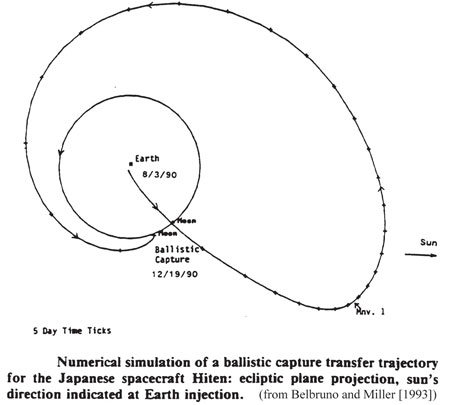
\includegraphics[width=0.60\linewidth]{fig/hiten.png}
    \caption{The Hiten spacecraft performed the first attempt at a LETO to the Moon ever in 1990, a 4 month trip that was a success (Image: \cite{Belbuno1990}).}
    \label{fig:hiten}
\end{figure}

After Hiten, a small number of missions have utilized LETOs in their missions \cite{Wikipedia}:
\begin{itemize}
	\item SMART-1 (ESA, 2003--2006): Was used to test solar electric propulsion and other deep-space technologies, while performing scientific observations of the Moon before deliberately crashing into it \cite{ESA}. Used electric propulsion to gradually make it's way to the moon.
    \item Genesis (NASA, 2001--2004): Collect solar wind samples at the Earth-Sun L1 Lagrange point and returned them to Earth for study \cite{NASAa}.
    \item GRAIL (NASA, 2011-2012): A pair of lunar orbiters that measured the gravitational field of the Moon very precisely, which could be used to infer the internal structure of the Moon. Entered into lunar orbit via a LETO very similar to Hiten \cite{NASA2013,Wikipediaa}. 
\end{itemize}

Since their discovery and usage in the 90's, the existence of a network of LETOs between planets in the solar system have been studied under the name ``Interplanetary Transport Network'' \cite{Ross2006}, although no concrete suggestions for actual advantageous LETO strategies to Mars was suggested until 2014.

\section{2014: Earth-Mars LETOs}
Earth-Mars LETOs have long thought to not be possible, but in 2014 this topic was explored in \cite{Topputo2014}. They proposed going to Mars in two steps:
\begin{enumerate}
	\item First a transfer orbit to a point $\mathrm{x}_c$ somewhere in the vicinity of Mars on the order of \SIrange{10e6}{10e7}{\km}, see \cref{fig:TransferStructure,fig:earth-mars-ballistic}.
	\item Then small delta-v applied at $\mathrm{x}_c$ to inject the spacecraft into the ballistic capture orbit.
\end{enumerate}

\begin{figure}[ht]
    \centering
    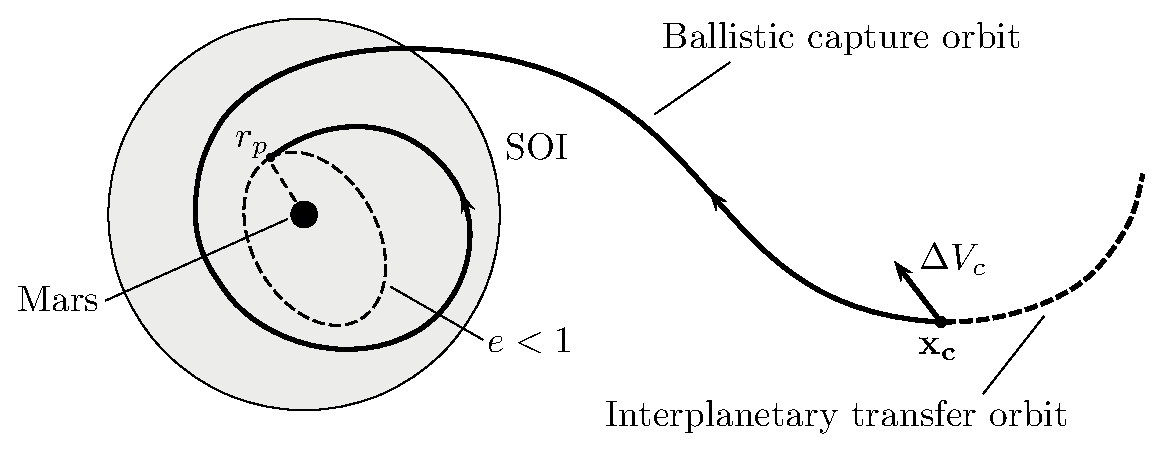
\includegraphics[width=0.70\linewidth]{fig/TransferStructure.eps}
    \caption{Structure of the ballistic capture transfers to Mars proposed by Topputo and Belbruno: First transfer to a point near mars, then make a ballistic capture (Image: \cite{Topputo2014}).}
    \label{fig:TransferStructure}
\end{figure}

\begin{figure}
    \centering
    \subfloat[An Earth-Mars ballistic capture in something resenbling a standard Hohmann transfer.]{
        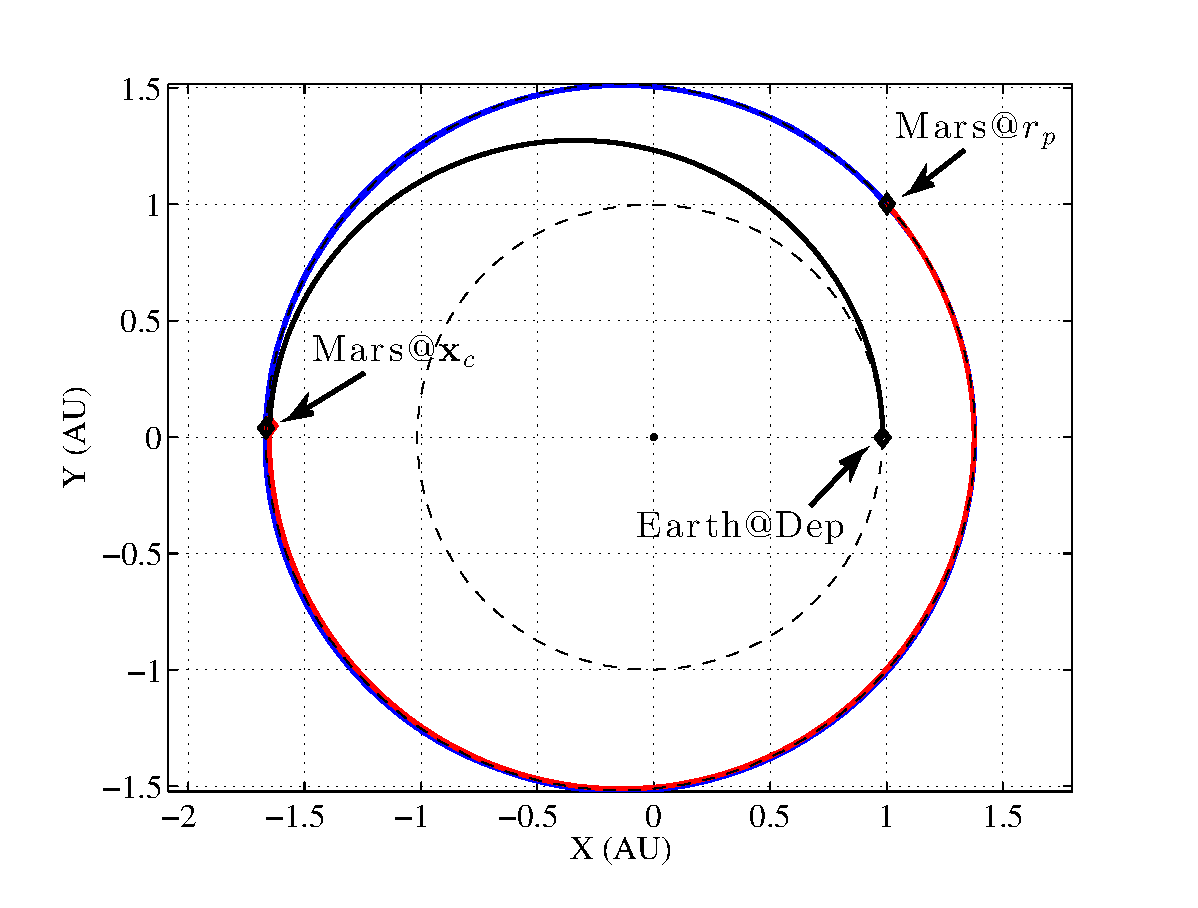
\includegraphics[width=0.47\linewidth]{fig/Sol1New.eps}
        \label{fig:earth-mars-ballistic-standard-hohmann}
    }
    \hfill
    \subfloat[An Earth-Mars ballistic capture at a different launch time with a much longer capture.]{
        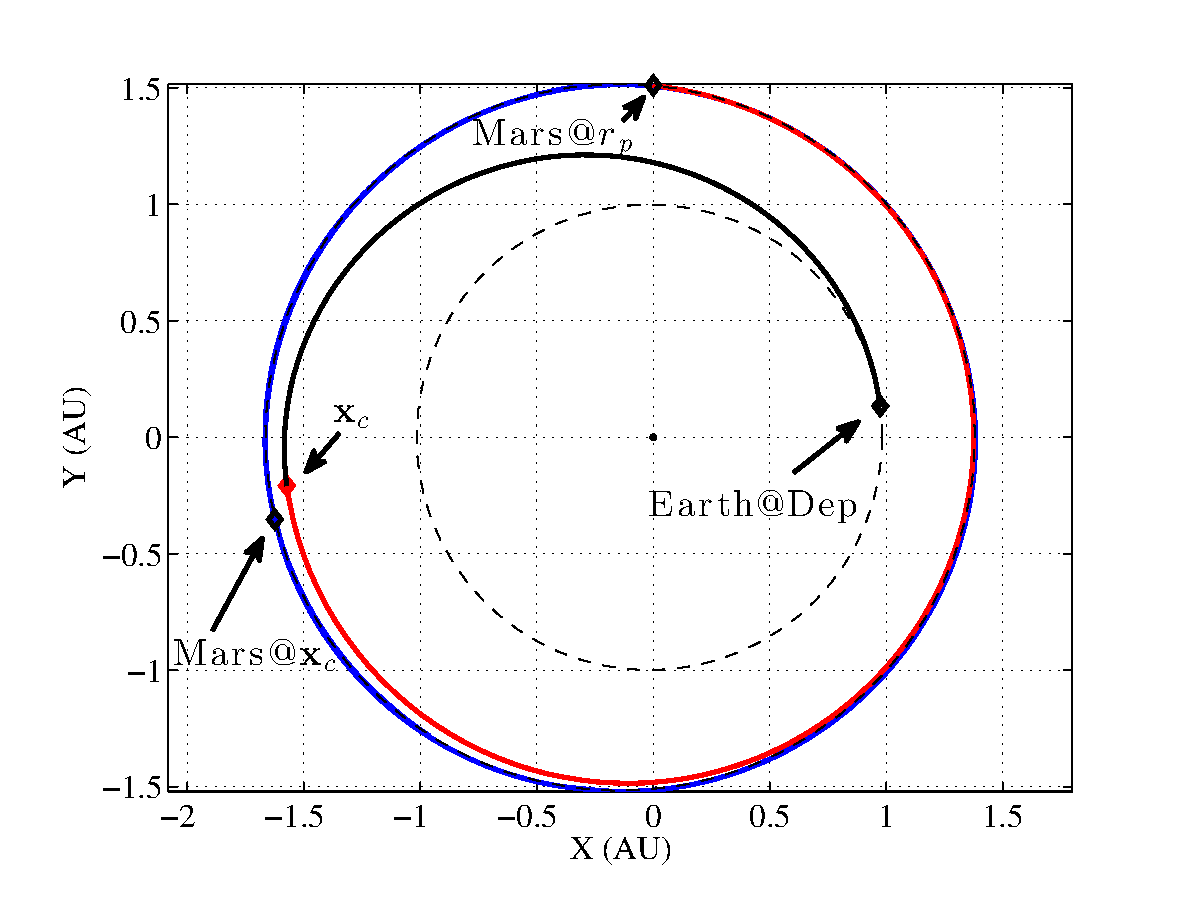
\includegraphics[width=0.47\linewidth]{fig/Sol12New.eps}
        \label{fig:earth-mars-ballistic-long-capture}
    }
    \caption{Two possible Earth-Mars LETOs, demonstrating the expanded launch window from Earth, an advantage over the standard Hohmann transfer (Image: \cite{Topputo2014}).}
    \label{fig:earth-mars-ballistic}
    \end{figure} 

However it is clear that this is still very early work, and the authors came to a couple of main conclusions:
\begin{enumerate}
	\item \textbf{Lower delta-v than Hohmann to Mars can be achieved}, but only for high-altitude orbits with apoapsis higher than \SI{22000}{\km}. The authors then simply postulate that goods can be delivered to low orbit or the surface easily, without any detail on how. It is not clear whether they consider aerobraking\footnote{A spacecraft maneuver that decreases the high point (apoapsis) of the orbit by flying through the atmosphere at the low point (periapsis) on the orbit, thereby slowing due to friction with the atmosphere.} a realistic option.
	\item \textbf{Expanded launch windows}, since the transfer orbit does not target one particular moving point (Mars) but many possible regions close to Mars. With a Hohmann transfer orbit, launches are limited to a few days every 26 months, but this type of Earth-Mars LETOs can be launched any time of the year, with varying trip times of up to a few years. However this is still faster than waiting more than 2 years for the next launch window for a traditional Hohmann \footnote{Incidentally, Belbruno have jokingly mocked the  movie ``The Martian'' for not taking LETOs to Mars into account when astronaut Mark Watney was stuck on Mars and badly in need of supplies from Earth \url{https://www.space.com/30749-the-martian-faster-way-to-mars.html}}.
	\item \textbf{Safer arrival conditions.} Topputo and Belbruno argues that their LETOs to Mars are in some sense safer than a Hohmann transfer due to the precise timing and high impulse required for the latter, whereas LETOs are more gradual in forgiving in nature and can tolerate temporary problems without being hurled into space or smashed into the surface of Mars.
\end{enumerate}
Whether these are convincing arguments to the wider community and organizations such as NASA and SpaceX remains to be seen. The first point above in particular seems to lack detail, and the authors admit that there is lots of work to be done in future studies on the topic.

However the paper did encourage us to proceed and try to find LETOs to Mars.

\section{Since the 1980's And  and Future: Novel Search Methods – Searching for LETOs Using Neural Networks and Evolution Strategies}
The literature on combining modern machine learning methods, such as neural networks or evolution strategies, goes back many years, even decades. \cite{Izzo2018} does a good job of providing an overview of the field of AI techniques applied to finding trajectories. However the field of AI as a whole has experienced a renaissance in the second decade of the 21st century, and the ever-increasing computing power have unlocked the potential of methods that once seemed intractable, such as Evolution Strategies \cite{Salimans2017} (to be introduced in \cref{sec:ES}).

``The use of machine learning (ML) algorithms to aid the design of interplanetary trajectory is not as widely researched as that of evolutionary techniques and is limited to fewer works. The reasons are to be found in the less obvious applicability of these methods to the problems encountered in the design of interplanetary trajectories and in the lack of data sets produced and made available by the aerospace community.'' \cite{Izzo2018}.

In 2016 \cite{Sanchez-Sanchez2016} explored using a deep neural network to learn the optimal control action for \emph{landing} a spacecraft, assuming perfect information. 

According to \cite{Izzo2018}, the last works in the cross-field of ML and interplanetary trajectories have all been limited to landing problems and the applicability of these ideas to interplanetary trajectories has not been studied before now. The authors concluded that ``It appears that a deep network is able to represent the optimal guidance structure of the Earth-Mars transfer quite satisfactorily introducing errors that are, on average, rather small.''.

In conclusion, the field of using evolutionary algorithms in the space of optimal trajectory search was surprisingly rich, but so was the variety of genetic algorithms applied. We therefore still found it worthwhile to experiment with the version treated in \cite{Salimans2017} (to be introduced in \cref{sec:ES}) and see what we could find.